\documentclass{llncs}
\usepackage{graphicx,color}
\usepackage{xspace}
\usepackage{amssymb} 
\usepackage{epstopdf}
\usepackage{algorithm} 
\usepackage{algorithmic}
\usepackage{caption}
\usepackage{subcaption}
     
% bibliography packages 
%\usepackage[nodots,nocompress]{numcompress}
\usepackage{multibib}
%Defining new way to cite
%\newcites{map}{Systematic Mapping References} 
%\usepackage{bibtopic}       
  
\usepackage{datatool}
\usepackage{tikz}
 
\usepackage{pgfplots}
\usepackage{pgfplotstable}
\pgfplotsset{compat=1.10}  

\usetikzlibrary{patterns}
\usepackage{lscape} 
\usepackage{subfig}
\usepackage{multirow}
\usepackage{rotating}

%  \usepackage{multibbl}
%  \usepackage{hyperref}



%% Use the option review to obtain double line spacing
%% \documentclass[preprint,review,12pt]{elsarticle}
   
%% Use the options 1p,twocolumn; 3p; 3p,twocolumn; 5p; or 5p,twocolumn
%% for a journal layout: 
%% \documentclass[final,1p,times]{elsarticle}
%% \documentclass[final,1p,times,twocolumn]{elsarticle}
%% \documentclass[final,3p,times]{elsarticle}
%% \documentclass[final,3p,times,twocolumn]{elsarticle}
%% \documentclass[final,5p,times]{elsarticle}
%% \documentclass[final,5p,times,twocolumn]{elsarticle}

%% if you use PostScript figures in your article
%% use the graphics package for simple commands
%% \usepackage{graphics}
%% or use the graphicx package for more complicated commands
%% \usepackage{graphicx}
%% or use the epsfig package if you prefer to use the old commands
%% \usepackage{epsfig}

%% The amssymb package provides various useful mathematical symbols
\usepackage{amssymb}

%% The amsthm package provides extended theorem environments
%%\usepackage{amsthm}

%\newtheorem{def}{Definition}

%% The lineno packages adds line numbers. Start line numbering with
%% \begin{linenumbers}, end it with \end{linenumbers}. Or switch it on
%% for the whole article with \linenumbers after \end{frontmatter}.
%% \usepackage{lineno}

%% natbib.sty is loaded by default. However, natbib options can be
%% provided with \biboptions{...} command. Following options are
%% valid:

%%   round  -  round parentheses are used (default)
%%   square -  square brackets are used   [option]
%%   curly  -  curly braces are used      {option}
%%   angle  -  angle brackets are used    <option>
%%   semicolon  -  multiple citations separated by semi-colon
%%   colon  - same as semicolon, an earlier confusion
%%   comma  -  separated by comma
%%   numbers-  selects numerical citations
%%   super  -  numerical citations as superscripts
%%   sort   -  sorts multiple citations according to order in ref. list
%%   sort&compress   -  like sort, but also compresses numerical citations
%%   compress - compresses without sorting
%%
%% \biboptions{comma,round}

% \biboptions{}


%\journal{Information and Software Technology}

%%% OUR MACROS %%%
%\newcommand{\COMMENT}[1]{ }

%\usepackage[usenames,dvipsnames]{xcolor}
\usepackage{xcolor}


\usepackage{amsmath}
\usepackage[thmmarks,amsmath]{ntheorem}

\newcommand{\openbox}{\leavevmode
  \hbox to.77778em{%
  \hfil\vrule
  \vbox to.675em{\hrule width.6em\vfil\hrule}%
  \vrule\hfil}}

\theoremstyle{plain}
\theoremheaderfont{\normalfont\bfseries}
\theorembodyfont{\normalfont}
\theoremseparator{}
\theoremindent0cm
\theoremnumbering{arabic}
\newtheorem{algo}{Algorithm}

\theoremstyle{plain}
%\theoremheaderfont{\normalfont\itshape}
\theoremheaderfont{\normalfont\bfseries}
\theorembodyfont{\normalfont}
\theoremseparator{}
\theoremindent0cm
\theoremnumbering{arabic}
\theoremsymbol{\ensuremath{\openbox}} 
%\newtheorem{example}{Example}


\theoremstyle{plain}
\theoremheaderfont{\normalfont\bfseries}
\theorembodyfont{\normalfont}
\theoremseparator{.}
\theoremindent0cm
\theoremnumbering{arabic}
\theoremsymbol{\ensuremath{\Box}} 
\newtheorem{defi}{Definition}

\theoremstyle{plain} 
\theoremsymbol{\ensuremath{\Box}} 
\theoremseparator{.} 
\newtheorem{prop}{Property}

\def\FlyingPig{\textsl{FlyingPig}}

\newcounter{numberInTrivlist}

\newenvironment{numtrivlist}{\begin{list}{\rm \arabic{numberInTrivlist})} 
                                         {\usecounter{numberInTrivlist}
                                          \setlength{\leftmargin}{0pt}
                                          \setlength{\rightmargin}{0pt}
                                          \setlength{\itemindent}{12pt}
                                          \setlength{\listparindent}{0pt}}}
                            {\end{list}}

\newenvironment{itemizedTrivlist}{\begin{list}{\rm ~\hspace{2mm} $\bullet$\ } 
                                         {\setlength{\leftmargin}{0pt}
                                          \setlength{\rightmargin}{0pt}
                                          \setlength{\itemindent}{12pt}
                                          \setlength{\listparindent}{0pt}}}
                            {\end{list}}

\usepackage{listings}


\lstset{numbers=right, numbersep=5pt, numberstyle=\tiny, stepnumber=1,escapechar=\!,columns=fullflexible,
        morekeywords={procedure,let,for,do,if,then,else,add,choose,end,while,
        true,false,rise,exception,extend,resume,to,return,function}}

\newcommand{\pisodm}[0]{$\pi$SOD-M\xspace}


\newcommand \tqI[1]{\hbox{${\cal T}_{\mathrm{init}} [\![\ #1\ ]\!]$}}
\newcommand \tqT[1]{\hbox{${\cal T}_{\mathrm{cond}} [\![\ #1\ ]\!]$}}
\newcommand \tqS[1]{\hbox{${\cal T}_{\mathrm{inc}} [\![\ #1\ ]\!]$}}
\newcommand \agg[1]{\ensuremath{{\cal A}{gg}(#1)}}


\def\P{\hbox{${\cal P}$}}
\def\bigLS{\hbox{${\cal L_{S}}$}}
\def\bigLCSD{\hbox{${\cal L_{CSD}}$}}
\def\bigS{\hbox{${\cal S}$}}
\def\bigV{\hbox{${\cal S}$}}
\def\V{\hbox{${S}$}}
\def\v{\hbox{${s}$}}
\def\MCDws{\ifmmode \mathit{COR\_D}\else \textit{COR\_D}\fi}

\renewcommand{\algorithmicrequire}{\textbf{Input:}}
\renewcommand{\algorithmicensure}{\textbf{Output:}}

\begin{document}
 
% ------ title and authors ----- % 

\title{\textit{Rhone}: a quality-based query rewriting algorithm for data
integration.}
\author{Daniel A. S. Carvalho\inst{1} \and Pl\'acido
		A. Souza Neto\inst{2} \and Chirine Ghedira-Guegan\inst{3} 
		\and Nadia Bennani\inst{4} \and Genoveva Vargas-Solar\inst{5} }
 
\institute{ 
Universit\'e Jean Moulin Lyon 3, Centre de Recherche Magellan, IAE, France\\
\email{daniel.carvalho@univ-lyon3.fr} \and
Instituto Federal do Rio Grande do Norte - IFRN, Natal, Brazil\\
\email{placido.neto@ifrn.edu.br} \and
Universit\'e Jean Moulin Lyon 3, LIRIS, Centre de Recherche Magellan, IAE,
France\\
\email{chirine.ghedira-guegan@univ-lyon3.fr} \and
LIRIS, INSA-Lyon, France\\
\email{nadia.bennani@insa-lyon.fr} \and
CNRS-LIG, Grenoble, France\\
\email{genoveva.vargas@imag	.fr} 
}

\maketitle

% ------ enf of title and authors ----- %
  
% ------ abstract and keywords ----- %
\begin{abstract}
Nowadays, data provision is mostly done by data services. Data integration can
be seen as composition of data services and data processing services that can
deal with to integrate data collections. With the advent of cloud, producing service compositions is
computationally costly. Furthermore, executing them can require a considerable
amount of memory, storage and computing resources that can be provided by
clouds. Our research focuses on how to enhance the results on the increase of cost on data integration in the new context of cloud.
To do so, we present in this paper our original data integration approach which takes into account user's
integration requirements while producing and delivering the results. The
service selection and service composition are guided by the service level
agreement - SLA exported by different services (from one or more clouds) and used by our matching algorithm (called \textit{Rhone}) that addresses the query rewriting for data integration presented here as proof of concept.
%The originality of  \textit{Rhone} is the rewriting process
%guided by quality measures associated to data providers (services) and user
%preferences. The paper uses a running scenario to describe the \textit{Rhone}'s
%formalization and its implementation. We also present an experimental
%evaluation. It shows that quality can be improved on data integration solutions.
%In addition, perspectives concerning our data integration approach and algorithm are presented.
%Data integration arises in the cloud computing as a service composition problem.
%Producing service compositions is computationally costly; and executing them require a considerable amount of memory, storage and computing resources.  
%Our research focus on how enhancing the quality on data integration in a cloud context.
%This paper presents a rewriting algorithm named \textit{Rhone} that addresses
%query for data integration. The originality of  \textit{Rhone} is the rewriting process
%guided by quality measures associated to data providers (services) and user
%preferences. The paper uses a running scenario to describe the \textit{Rhone}'s
%formalization and its implementation. We also present an experimental
%evaluation. It shows that quality can be improved on data integration solutions.
%In addition, perspectives concerning our data integration approach and algorithm are presented.
\end{abstract}
 
\keywords{Data integration. Query rewriting. Query rewriting algorithm. Cloud computing. SLA.}
 
% ------ end of abstract and keywords ----- %

\section{Introduction}\label{sec:introduction}
%Integrating data across different databases, and provide an unique view of it to the user, is a problem in the database domain (called data integration).
Data integration problem has been studied by many researchers in the database domain.
This can be seen in the service-oriented architecture as a service composition issue, such as given a query, the objective is to lookup for data services and compose them in order to achieve a desired result. 
%
%Finding the best service composition to answer a query can be computationally costly. 	
However, it is computationally costly to find the best service composition to answer a query. 
Furthermore, executing the composition can lead to retrieve and process data collections that can require important memory, storage and computing resources.
The on-demand resource provision imposed by the cloud computing architecture opens challenges to data processing and management.
%The cloud architecture allows and opens challenges to the data integration once such architecture give us an unlimited access to resources. 
%The possibility of having an unlimited access to resources, the resource management, the geographically distributed location of services, and the economic model imposed by the cloud architecture open challenges to data integration solutions.
Data integration has evolved with the emergence of data services that
deliver data under different quality conditions related to data freshness, cost, reliability,
availability, among others. Data are produced continuously and on demand in huge
quantities and sometimes with few associated meta-data, which makes the
integration process more challenging. Some approaches express data integration
as a service composition problem where given a query the objective is to lookup
and compose data services that can contribute to produce a result. Finding the
best service composition that can answer a query can be computationally costly.
Furthermore,  executing the composition can lead to retrieve and process data
collections that can require important memory, storage and computing resources.     

This problem has been addressed in the service-oriented
domain~\cite{Barhamgi2010,Benouaret2011,ba2014}.
Generally, these solutions deal with query rewriting problems.
\cite{Barhamgi2010} proposed a query rewriting approach which processes queries
on data provider services. \cite{Benouaret2011} introduced a service composition
framework to answer preference queries. In that approach, two algorithms based
on~\cite{Barhamgi2010} are presented to rank the best rewritings based on previously computed scores.
\cite{ba2014} presented an algorithm that produces and order rewritings
according to user preferences. Yet, to our knowledge few works consider quality
measures associated both to data services and to user preferences in order to
guide the rewriting process. 

Computing resources are delivered as services by the cloud. Services are billed and agreed between service providers and service customers under service level agreement (SLA) contracts.
Both sides must agree together on quality conditions and penalties under which the service is delivered. 
%Generally, those conditions and penalties associated to its violation are defined in service level agreement (SLA). 
Several researches have reported their studies on SLA in different domains~\cite{AlhamadDC11}.
SLA proposals for cloud computing could be divided in two groups: (i) works developing tools and methods to help on SLA negotiation and enforcement phase~\cite{rak2013,Mavrogeorgi2013}; and (ii) approaches that monitor contracts and cloud resources in order to detect and avoid SLA violations~\cite{Leitner2010,Maarouf2015}. To our knowledge, SLA publications have not been yet integrated to data integration in a multi-cloud environment.

Based on these concepts and open challenges, the goal of this work is to present
a data integration solution concerning a service-based query rewriting algorithm guided by SLA's.
Our work addresses these issues and proposes the algorithm (we
called \textit{Rhone}) with two original aspects: (i) the user can express her
quality preferences and associate them to her queries; and (ii)  service's quality aspects defined on Service Level Agreements (SLA) guide service selection and the whole rewriting process.
Yet, to the best of our knowledge, we have not identified any other work that uses SLA to guide the entire data integration solution.

This paper is organized as follows. Section ~\ref{sec:disla} discusses
about data integration and service level agreements (SLA).
Section~\ref{sec:scenario} contains the running scenario and challenges.
Section~\ref{sec:relatedwork} presents some related works.
Section~\ref{sec:rhone} describes the \textit{Rhone} algorithm and its
formalization.
Experiments and results are described in the section~\ref{sec:experiments}. 
Finally, section~\ref{sec:conclusion} concludes the paper and discusses future works.

\section{Related works}\label{sec:relatedwork}
In recent years, the cloud have been the most popular deployment environment for data integration~\cite{Carvalho2015}. Existing works addressing this issue can be grouped according to two different lines of research:
\textit{(i)} data integration and services~\cite{Correndo2010,ElSheikh2013,Tian2010,YauY08}; and
\textit{(ii)} service level agreements (SLA) and data integration~\cite{Bennani2014,Nie07}. 

\cite{Correndo2010} proposed a query rewriting method for achieving RDF data integration. % using SPARQL. The principle of the approach is to rewrite the RDF graph pattern of the query using data manipulation functions in order to: (i) solve the entity co-reference problem which can lead to ineffective data integration; and (ii) exploit ontology alignments with a particular interest in data manipulation. 
The objective of the approach is to: (i) solve the entity co-reference problem which can lead to ineffective data integration; and (ii) exploit ontology alignments with a particular interest in data manipulation. 
\cite{ElSheikh2013} introduced a system (called SODIM) which combines data integration, service-oriented architecture and distributed processing. %SODIM works on a pool of collaborative services and can process a large number of databases represented as web services. 
The novelty of these approaches is that they perform data integration in service oriented contexts, particularly considering data services. They also take into consideration the requirement of computing resources for integrating data. Thus, they exploit parallel settings for implementation costly data integration processes. 

A major concern when integrating data from different sources (services) is privacy that can be associated to the conditions in which integrated data collections are built and shared.
\cite{YauY08} focused on data privacy based on  a privacy preserving repository in order to integrate data. 
Based on users' integration requirements, the repository supports the retrieval and integration of
data across different services. 
\cite{Tian2010} proposes an inter-cloud data integration system that considers a trade-off between users' privacy requirements and the cost for protecting and processing data. According to the users' privacy requirements, the query plan in the cloud repository creates the users' query. This query is subdivided into sub-queries that can
be executed in service providers or on a cloud repository. Each option has its own  privacy and processing costs.
Thus, the query plan executor decides the best location to execute the sub-query to meet privacy and cost constraints.

Service level agreement (SLA) contracts have been widely adopted in the context of Cloud computing. Research contributions mainly concern (i) SLA negotiation phase (step in which the contracts are established between customers and providers) and (ii) monitoring and allocation of cloud resources to detect and avoid SLA violations.
\cite{Nie07} proposed a data integration model guided by SLAs in a grid environment. Their architecture is subdivided into four parts: (i) a SLA-based resource description model describes the database resources; (ii) a SLA-based query model normalizes the different queries based on the SLA; (iii) a SLA-based matching algorithm selects the databases; and finally (iv) a SLA-based evaluation model obtains the final query solution.
Apart from our previous work~\cite{Bennani2014}, to the best of our knowledge, there is no evidence of researches on SLA applied to data integration in a (multi-)cloud context.

The main aspect in a data integration solution is 
the query rewriting process executed by a mediator
in accordance with the different databases.
%
In this way, algorithms for rewriting queries have
been proposed in two domains: (i) on the database 
domain; and (ii) on the service-oriented domain.

On the database domain, query rewriting approaches using
views have been widely discussed~\cite{Halevy:2001}.
%
For instance, the \textit{bucket algorithm}~\cite{Levy:1996}, 
\textit{inverse-rules algorithm}~\cite{Duschka:1997} and 
\textit{MiniCon algorithm}~\cite{Pottinger:2001} have
tackled the rewriting problem on the database domain.
%
In addition, \cite{Pottinger:2001} has inspired rewriting methods in service-oriented domain~\cite{costa2013,ba2014}.
%In addition, these algorithms have also inspired other algorithms in the database and service-oriented domains♣~\cite{costa2013} (REF THE WORKS).
%These approaches will not be detailed here once the focus
%of this paper is on algorithms in the service-oriented domain.

%Generally, data integration solutions on the service-oriented domain deal with query rewriting problems.
Data integration solutions on the 
service-oriented domain deal with query rewriting problems. \cite{Carvalho2015} identifies
trends and open issues regarding the use of SLA in data integration solutions on
multi-cloud environments.
%
\cite{Barhamgi2010} proposes a query rewriting approach 
which processes queries on data provider services.
The query and data services are modeled as RDF views.
A rewriting answer is a service composition in which 
the set of data service graphs fully satisfy the query graph.  
%
\cite{Benouaret2011} introduces a service composition
framework to answer preference queries. In that approach, two algorithms based
on~\cite{Barhamgi2010} are presented to rank the best rewritings based on previously computed scores.
%
\cite{ba2014} presents an algorithm based on \textit{MiniCon} 
that produces and order rewritings according to user preferences. 
The user preferences on this approach are scores used to rank 
services that should be previously define by the user. 
%
Considering the scenario presented in the previous section and the related works
discussed in this one, we identify a gap between the application of quality
measures in the context of data integration domain. Thus, the main
and original proposal of our work is to use SLA to guide the entire data integration process.

Our approach differs from these works in three aspects:
(i) the user can express quality measures and associate them
to his queries, such as: \textit{I want to use services with response
time less than 2 seconds, price per request less than 1 dollar
and location close to my city}; 
(ii) the user preferences guides the service selection. 
These preferences are matched with the services' quality aspects
that are extracted from service level agreement contracts.
Here, it is important to highlight that there
is a previous phase in which the services' quality aspects are 
processed and extracted from SLAs. 
In our proposal we are assuming that these information are accessible and
well-formatted to the algorithm; and
(iii) the user preferences are also used to guide the rewriting process.
The rewriting answers (services compositions) produced must be in 
accordance with the user preferences.
%

% Yet, to the best of our knowledge, few works consider quality
% measures associated both to data services and to user preferences in order to
% guide the rewriting process, and there is no approach using SLAs to guide the
% data integration solution. 

%Here, it is important to highlight that this paper focus on the description and
%evaluation of the algorithm that rewrites queries in terms of services
%composition taking into account user preferences and service quality aspects
%expressed in SLA contracts. We are assuming that the extraction of quality
%aspects from SLAs is performed in a previous phase of our global data
%integration solution. 
%In the next section, the Rhone service-based algorithm is described and
%formalized.

\section{SLA guided data integration in cloud evironments}\label{sec:scenario}
%This section is devoted to describe the motivation scenario %and challenges
concerning our data integration approach.
%

Let us assume the following scenario in the medical domain. 
Users are able to retrieve information about (i) patients that were infected by a disease; 
(ii) regions most affected by a disease in Europe; 
(iii) patients' personal information; and 
(iv) patients' dna information.
To perform these actions, four family of services are necessary: family
\textbf{A} has services which given a disease name, it retrieves the list
of infected patients; family \textbf{B} has services which given a disease name,
it retrieves the list of cities most affected by that disease; family \textbf{C}
has services which given a patient id, it retrieves patients' personal
information; and family \textbf{D} has services which given a patient id, it
retrieves patients' dna information. 

Doctor Marcel would like to study the type of people suffering of a
particular disease. For instance, he needs to query the patients' personal
information and patients' dna information from the set of patients that were
infected by flu. Presuming that Marcel has at his disposal a cloud
including a set of services from the families \textbf{A}, \textbf{B}, \textbf{C} and \textbf{D}. To achieve
his needs, Marcel can use the data services as follows: (i) he invokes service
\textbf{S1} (family \textbf{A}) with the disease information then he gets the
set of people infected by flu; (ii) then he invokes service \textbf{S2} (family
\textbf{C}) with the obtained patients in order to retrieve their personal
information; just after (iii) Doctor Marcel invokes service \textbf{S3} (family
\textbf{D}) with the obtained patients to retrieve their dna information.
Finally, the query results is integrated and returned.

Depending on the amount of services in each family type, a lot of other service 
compositions could be done to answer Marcel's query. A large quantity of
algorithms for this purpose have been developed, and all of them share the same
problems: (1) producing rewritings when a big amount of services are available
is extremely expensive; and (2) not always the quality of the rewriting (composition) produced is enough for meeting your needs.
Motivated by these problems, our approach proposes a new vision of data
integration as follows.

Assuming the same medical scenario and the same families of data services.
Let us suppose Marcel would like to study the type of people suffering of a
particular disease as before. However, in this new scenario, he is also capable
to express his preferences while integrating services. For instance, he needs to
query the patients' personal information and patients' dna information from
patients that were infected by flu, using services with availability higher than
98\%, price per call less than 0.2\$ and total cost less than 2\$. Marcel has at his disposal a set of services from the families \textbf{A}, \textbf{B}, \textbf{C} and \textbf{D} geographically disposed on different cloud provides (configuring a multi-cloud environment).
To achieve his needs, Marcel can use the data services as before invoking one
service from the families \textbf{A}, \textbf{C} and \textbf{D} in sequence.
However, in this new configuration all the services involved must satisfy the
user preferences expressed in the query. The selection and rewriting process is
guided by the service level agreements (SLA) exported from different services.
The user preferences are matched with the service quality aspects that are
defined on its SLAs.     

This vision of data integration brings some reflections and questions
considering the challenges presented previously, such as:
(i) The amount of services involved in a multi-cloud context is bigger than in a
single cloud. Consequently, the number of services that can be used in the
rewriting process and the number of rewriting produced is higher. Such
environment calls for a better services selection process, \textit{i.e.}, guided
by the SLAs and user preferences; (ii) How can the different SLAs associated to
services and cloud provider can be integrated with the user preferences? There
are different levels of SLAs: the one agreed between services and cloud
providers; and the ones agreed between services and users. These SLAs should be
integrated; and (iii) How can a previous processed query be reused for a next query?

% Here, it is important to highlight that this paper focus on the description and
% evaluation of the algorithm that rewrites queries in terms of services
% composition taking into account user preferences and service quality aspects
% expressed in SLA contracts. We are assuming that the extraction of quality
% aspects from SLAs is performed in a previous phase of our global data integration solution.
In the next section we are going to discuss the related works concernig data
integration and service level agreements, in order to identify the gap between
the presented challenges and how the works address these problems.

With the advent of cloud and multi-clouds a new vision of data integration is to be considered.
In this vision 
(i) \textit{data services} provide access and allow data retrieval;  
(ii) \textit{data processing services} retrieve and process data; 
(iii) \textit{data services} and \textit{data processing services} can be deployed in different \textit{cloud providers} geographically distributed; 
(iv) \textit{data services}, \textit{data processing services} and the \textit{cloud} itself export their SLA defining the services they provide and the quality conditions under which they are delivered. Different levels of SLA are considered: contracts agreed between \textit{data services} or \textit{data processing services} and \textit{cloud providers}, called \textit{cloud SLA} (SLA$_{C}$); and contracts agreed between users and \textit{data services} or \textit{data processing services}, called \textit{service SLA} (SLA$_{S}$). 
Therefore, given a user query, his/her integration quality requirements and his/her cloud subscription, the query is rewritten in terms of cloud services (\textit{data services} and \textit{data processing services}) composition that fulfill the integration requirements and deliver the expected results to the user.
%The figure~\ref{fig:scenario} illustrates our data integration vision.

% \begin{figure}[h!]
% \center
% 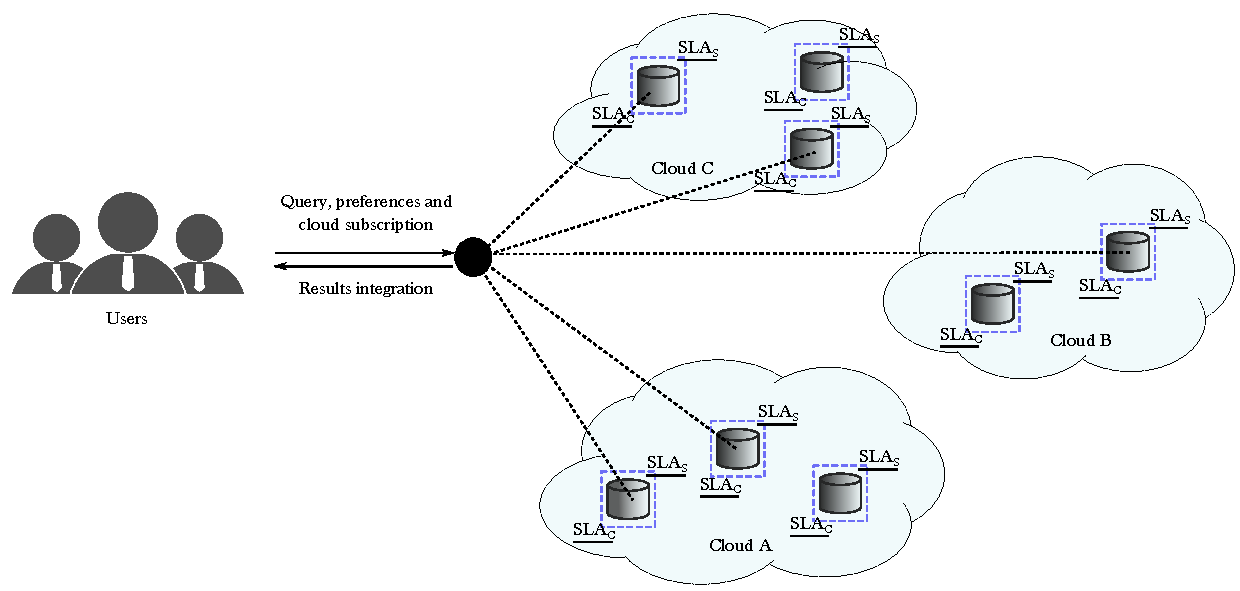
\includegraphics[scale=0.57]{scenario.pdf}
% \caption{New vision of data integration}\label{fig:scenario}
% \end{figure}

To better understand our vision and challenges, let us consider the following medical scenario in which users are able to retrieve and integrate data concerning (i) \textit{patients that were infected by a disease;}
(ii) \textit{regions most affected by a disease}; (iii) \textit{patients' personal information}; and (iv) \textit{patients' DNA information}. For instance, doctor \textit{Marcel} would like to study the type of people suffering of \textit{flu} in the Europe. To perform this, he has at his disposal a set of cloud services delivered by different \textit{cloud providers}.
Each cloud service and \textit{cloud provider} describe their quality guarantees in SLA contracts. Thereby, to reach his needs, he wants to query the personal and DNA information from patients infected by \textit{flu}, using cloud services with availability higher than 98\%, price per call less than 0.2\$ and integration total cost less than 5\$. This scenario introduces new challenges to data integration that have to be addressed, such as:
\begin{itemize}
\item Data integration tasks can require a huge amount of resources and processing time given the large quantity of \textit{data services} and \textit{data processing services};
\item The cloud model comes with the possibility of an on-demand and pay-per-use access to resources. However, cloud consumers have a restricted to the resources according to the contract they have with the cloud, and to the budget they are ready to pay while integrating data.
\item Part of the rewritings produced and executed to the user \textit{query} could not be in accordance with her quality requirements. In addition, generating these unsatisfactory rewritings imply increasing  the processing time and integration cost. Consequently, the user may become dissatisfied with the results. 
\item Performing data integration in this scenario implies a matching problem of users' requirements with different services' guarantees specified in SLAs. Considering the multi-cloud environment, we can face different cases of SLA incompatibilities given the different semantics and structure of SLAs exported by the different cloud services and \textit{cloud providers}.
\item Executing data integration tasks is computationally costly in terms of processing time and economic cost. Therefore, it is crucial to reuse previous integration results in order to save time and money while satisfying the user.
\end{itemize}

Motivated by the challenges discussed above, the figure~\ref{fig:workflow} illustrates our SLA-based data integration workflow. Given a user query, a set of user preferences associated to it, cloud providers and cloud services, the workflow can be divided in four steps:

\begin{figure}[h!]
\center
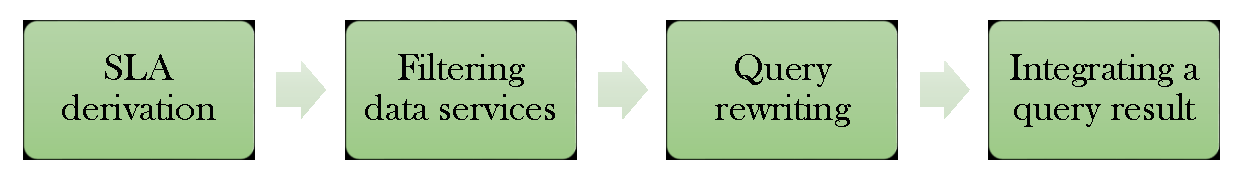
\includegraphics[scale=0.50]{workflow-approach.pdf}
\caption{SLA-based data integration workflow}\label{fig:workflow}
\end{figure}

\noindent \textbf{\underline{SLA derivation}}. In this step, we compute what we call a \textsl{derived SLA} that matches user' integration requirements (including quality constraints and data requirements) with the SLA's provided by \textit{cloud services}, given a specific user cloud subscription. The user may have general \textit{preferences} depending on the context he/she wants to integrate his/her data such as economic cost, bandwidth limit, free services, and storage and processing limits. The \textit{SLA derivation} is the big challenge while dealing with SLAs and particularly for adding quality dimensions to data integration. Furthermore, the \textsl{derived SLA} guides the query evaluation, and the way results are computed and delivered. \\
\textbf{\underline{Filtering data services}}. The \textsl{derived SLA} is used (i)
to filter previous \textsl{integration SLA} derived for a similar request in order to reuse results; or (ii) to filter possible \textit{cloud services} that can be used for answering the query. \\ %The SLA exported by a selected \textit{cloud service} should satisfy the user \textit{preferences}. \\
\textbf{\underline{Query rewriting}}. Given a set of \textit{data services} that can
potentially provide data for integrating the query result, a set of service compositions is generated according to the \textsl{derived SLA} and the agreed SLA of each \textit{data services}. \\
\textbf{\underline{Integrating a query result}}. The service compositions are
executed with services from one or several clouds where the user has a
subscription.
The execution cost of service compositions must fulfill the \textsl{derived
SLA}. The clouds resources needed by the user to execute the composition and how
to use them is decided taking in consideration the economic cost determined by
the data to be transferred, the number of external calls to services, data storage and delivery cost.

Although \textit{the SLA derivation} is the big challenge while dealing with
SLAs and particularly for adding quality dimensions to data integration, the
focus in this paper is our query rewriting algorithm which deals with user
preferences and SLAs exported by different cloud providers and data services.
Here, we are assuming that there is a mechanism responsible to extract the
services' quality aspects from SLA, and to provide this information as input to
the algorithm. The figure~\ref{fig:cloudsla} illustrates the structure of SLA
and its measures that are considered in the algorithm we will detail in the next
section.   

\begin{figure}[h!]
\center
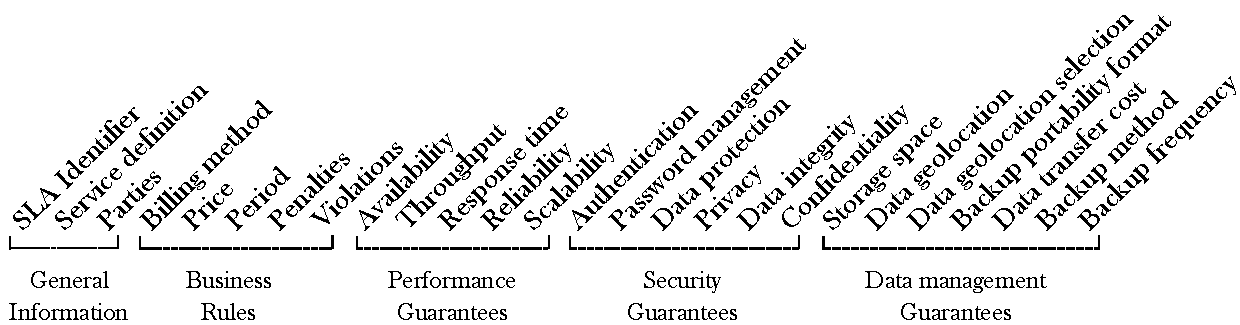
\includegraphics[scale=0.57]{Cloud_SLA.pdf}
\caption{Cloud SLA}\label{fig:cloudsla}
\end{figure}
%\section{SLA guided data integration}\label{sec:disla}
%
Motivated by the problems highlighted, we propose a new vision of data integration.

%In this scenario, depending on the amount of services available to Marcel, many service compositions could be produced to answer \textit{Marcel}'s query. AA large quantity of
%algorithms for this purpose have been developed, and all of them share the same
%problems: (1) producing rewritings when a big amount of services are available
%is extremely expensive; and (2) not always the quality of the rewriting (composition) produced is enough for meeting your needs.
%Motivated by these problems, our approach proposes a new vision of data
%integration as follows.

Assuming the medical scenario and \textit{Marcel}'s interest in the type of people
suffering of the particular disease, he can be
also capable to express his preferences while integrating services. For instance, he needs to query the patients' personal information and patients' DNA information from patients that were infected by flu, using services with availability higher than 98\%, price per call less than 0.2\$ and total cost less than 2\$.
\textit{Marcel} has at his disposal a set of services \textbf{S1}, \textbf{S2}, \textbf{S3} and \textbf{S4} geographically disposed on different cloud provides (configuring a multi-cloud environment).
To achieve his needs, \textit{Marcel} can use the data services as before invoking in sequence the service \textbf{S1}, \textbf{S3} and \textbf{S4}. However, in this new context, the service selection and rewriting process should meet the user' requirements.   

%This vision of data integration brings some reflections and questions considering the challenges presented previously, such as: (i) The amount of services involved in a multi-cloud context is bigger than in a single cloud. Consequently, the number of services that can be used in the rewriting process and the number of rewriting produced is higher. Such environment calls for a better services selection process, \textit{i.e.}, guided by the SLAs and user preferences; (ii) How can the different SLAs associated to services and cloud provider can be integrated with the user preferences? There are different levels of SLAs: the one agreed between services and cloud providers; and the ones agreed between services and users. These SLAs should be integrated; and (iii) How can a previous processed query be reused for a next query?

%Assuming the same medical scenario and the same families of data services.
%Let us suppose \textit{Marcel} would like to study the type of people suffering of a
%particular disease as before. However, in this new scenario, he is also capable
%to express his preferences while integrating services. For instance, he needs to
%query the patients' personal information and patients' dna information from
%patients that were infected by flu, using services with availability higher than
%98\%, price per call less than 0.2\$ and total cost less than 2\$. \textit{Marcel} has at his disposal a set of services from the families \textbf{A}, \textbf{B}, \textbf{C} and \textbf{D} geographically disposed on different cloud provides (configuring a multi-cloud environment).
%To achieve his needs, \textit{Marcel} can use the data services as before invoking one
%service from the families \textbf{A}, \textbf{C} and \textbf{D} in sequence.
%However, in this new configuration all the services involved must satisfy the
%user preferences expressed in the query. The selection and rewriting process is
%guided by the service level agreements (SLA) exported from different services.
%The user preferences are matched with the service quality aspects that are
%defined on its SLAs.     
%
%This vision of data integration brings some reflections and questions
%considering the challenges presented previously, such as:
%(i) The amount of services involved in a multi-cloud context is bigger than in a
%single cloud. Consequently, the number of services that can be used in the
%rewriting process and the number of rewriting produced is higher. Such
%environment calls for a better services selection process, \textit{i.e.}, guided
%by the SLAs and user preferences; (ii) How can the different SLAs associated to
%services and cloud provider can be integrated with the user preferences? There
%are different levels of SLAs: the one agreed between services and cloud
%providers; and the ones agreed between services and users. These SLAs should be
%integrated; and (iii) How can a previous processed query be reused for a next query?

% Here, it is important to highlight that this paper focus on the description and
% evaluation of the algorithm that rewrites queries in terms of services
% composition taking into account user preferences and service quality aspects
% expressed in SLA contracts. We are assuming that the extraction of quality
% aspects from SLAs is performed in a previous phase of our global data integration solution.
%In the next section we are going to discuss the related works concerning data
%integration and service level agreements, in order to identify the gap between
%the presented challenges and how the works address these problems.

%In recent years, the cloud have been the most popular deployment environment for data integration~\cite{Carvalho2015}. Existing works addressing this issue can be grouped according to two different lines of research:
%\textit{(i)} data integration and services~\cite{Correndo2010,ElSheikh2013,Tian2010,YauY08}; and
%\textit{(ii)} service level agreements (SLA) and data integration~\cite{Bennani2014,Nie07}. 
%
%\cite{Correndo2010} proposed a query rewriting method for achieving RDF data integration. % using SPARQL. The principle of the approach is to rewrite the RDF graph pattern of the query using data manipulation functions in order to: (i) solve the entity co-reference problem which can lead to ineffective data integration; and (ii) exploit ontology alignments with a particular interest in data manipulation. 
%The objective of the approach is to: (i) solve the entity co-reference problem which can lead to ineffective data integration; and (ii) exploit ontology alignments with a particular interest in data manipulation. 
%\cite{ElSheikh2013} introduced a system (called SODIM) which combines data integration, service-oriented architecture and distributed processing. %SODIM works on a pool of collaborative services and can process a large number of databases represented as web services. 
%The novelty of these approaches is that they perform data integration in service oriented contexts, particularly considering data services. They also take into consideration the requirement of computing resources for integrating data. Thus, they exploit parallel settings for implementation costly data integration processes. 
%
%A major concern when integrating data from different sources (services) is privacy that can be associated to the conditions in which integrated data collections are built and shared.
%\cite{YauY08} focused on data privacy based on  a privacy preserving repository in order to integrate data. 
%Based on users' integration requirements, the repository supports the retrieval and integration of
%data across different services. 
%\cite{Tian2010} proposes an inter-cloud data integration system that considers a trade-off between users' privacy requirements and the cost for protecting and processing data. According to the users' privacy requirements, the query plan in the cloud repository creates the users' query. This query is subdivided into sub-queries that can
%be executed in service providers or on a cloud repository. Each option has its own  privacy and processing costs.
%Thus, the query plan executor decides the best location to execute the sub-query to meet privacy and cost constraints.
%
%Service level agreement (SLA) contracts have been widely adopted in the context of Cloud computing. Research contributions mainly concern (i) SLA negotiation phase (step in which the contracts are established between customers and providers) and (ii) monitoring and allocation of cloud resources to detect and avoid SLA violations.
%\cite{Nie07} proposed a data integration model guided by SLAs in a grid environment. Their architecture is subdivided into four parts: (i) a SLA-based resource description model describes the database resources; (ii) a SLA-based query model normalizes the different queries based on the SLA; (iii) a SLA-based matching algorithm selects the databases; and finally (iv) a SLA-based evaluation model obtains the final query solution.
%Apart from our previous work~\cite{Bennani2014}, to the best of our knowledge, there is no evidence of researches on SLA applied to data integration in a (multi-)cloud context.

%\section{SLA guided data integration}
%Given a user query, a set of user preferences associated to it, cloud providers and services, our SLA guided data integration process can be divided in four steps. %The figure 1 illustrates our data integration approach.
%
%\begin{figure}[h!]
%\center
%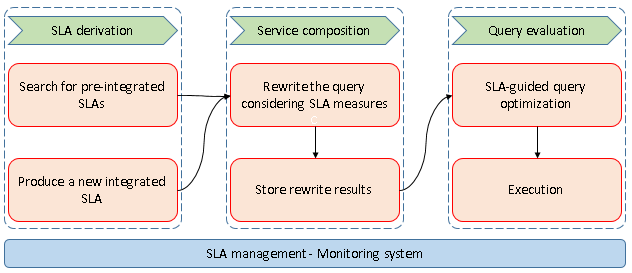
\includegraphics[scale=0.7]{general_approach.PNG}\label{fig:approach}
%\caption{SLA-guided data integration approach}
%\end{figure}

%\underline{The first phase} is the SLA derivation in which a SLA for the user request is created. It consists in looking for a (stored, integrated) SLA derived for a similar request. If a similar SLA is found, the request is forwarded to the query evaluation phase. Otherwise, a new SLA to the integration (called integrated SLA) is produced. The query is expressed as a service composition with associated user preferences. In \underline{the second phase}, service composition, the query is rewritten in terms of different services considering the user preferences and the SLAs of each service involved in the composition. The rewriting result is stored for further uses. \underline{Finally}, in the query evaluation phase, the query is optimized in terms of user preferences and SLAs concerning the consumed resources and the economic cost of the query. Once optimized, the query processed in the execution engine. In addition, we are assuming a SLA management module and monitoring system responsible to verify if the SLA contracts are being respected. Firstly, we have worked on the phases two in order to have an algorithm that will allow us to run important experiments to evaluate our approach. 
Thus, given a user query, a set of user preferences associated to it, cloud
providers and services, a SLA guided data integration process can be divided in four steps.
\bigskip

\noindent \underline{1. SLA derivation}. This step creates an \textsl{integrated
SLA} that includes a set of measures corresponding to the user preferences. The \textsl{integrated SLA} guides the query evaluation, and the way results are computed and delivered. \\
\underline{2. Filtering data services}. The \textsl{integrated SLA} is used (i)
to filter previous SLA derived for a similar request in order to reuse previous results; or (ii) to filter possible data services that can be used for answering the query. \\
\underline{3. Query rewriting}. Given a set of data services that can
potentially provide data for integrating the query result, a set of service compositions is generated according to the \textsl{integrated SLA} and the agreed SLA of each data service. \\
\underline{4. Integrating a query result}. The service compositions are executed
in one or several clouds where the user has a subscription. The execution cost of service compositions must fulfill the \textsl{integrated SLA} (that expresses user requirements). Here, the clouds resources needed to execute the composition and how to use them is decided taking in consideration the economic cost determined by the data to be transferred, the number of external calls to services, data storage and delivery cost.
\bigskip

Although \textit{the SLA derivation} is the big challenge while dealing with
SLAs and particularly for adding quality dimensions to data integration, the
focus in this paper is our query rewriting algorithm which deals with user
preferences and SLAs exported by different cloud providers and data services.
Here, we are assuming that there is a mechanism responsible to extract the
services' quality aspects from SLA, and to provide this information as input to
the algorithm. 

%The first phase is an open issue for dealing with SLAs and particularly for adding quality dimensions to  data integration. The problem is complex because SLA describe different elements participating in the data integration process: data services, cloud services at the different levels of the architecture (i.e., IaaS, PaaS, SaaS), data consumers subscriptions to cloud providers. The SLAs contain measures related to the way services are provided but also related to the data they provide. All these aspects must be considered for matching resources (i.e., services) with data consumers preferences. As shown in the following section and in our study SLA models and languages have been proposed. In contrast  efficient preferences and SLAs matching algorithms need to be proposed to compute derived SLAs. Concerning the other data integration phases, they have been partially addressed by existing works, where some quality dimensions are considered (e.g., data privacy). In our vision there are open issues to be addressed in order to have solutions that consider SLA in order to enhance data integration in multi-cloud environments. 

\begin{figure}[h!]
\center
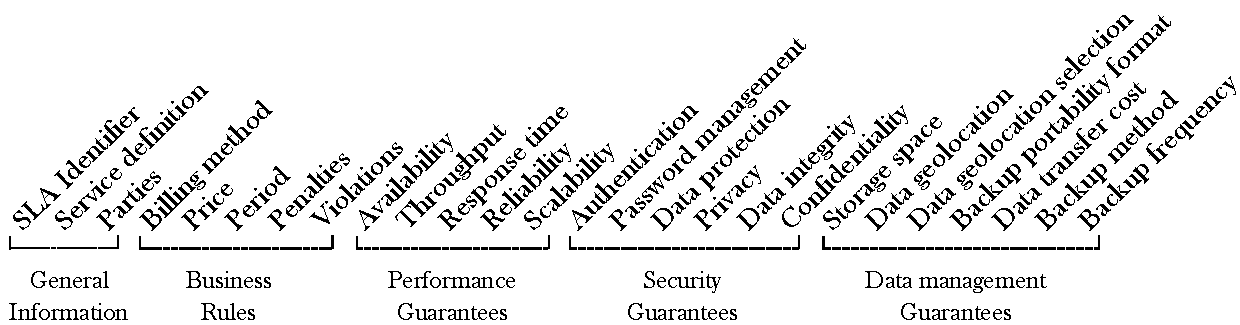
\includegraphics[scale=0.57]{Cloud_SLA.pdf}
\caption{Cloud SLA}\label{fig:cloudsla}
\end{figure}

The figure~\ref{fig:cloudsla} illustrates the structure of SLA
and its measures that are considered in the approach we will detail in the next
section.
\section{Rhone service-based query rewriting algorithm}\label{sec:rhone}
\textcolor{red}{Introduzir e descrever o algoritmo. Depois iniciar a formalizacao...}
The input for the \textit{Rhone} algorithm is: (1) a query; (2) a list of concrete services.

\begin{definition}[queries]
A query $Q$ is defined as a set of \textit{abstract services}, a set of \textit{constraints}, and a set of \textit{user preferences} in accordance with the grammar:
%
\begin{center}
\small
\begin{math}
Q (\overline{I}_{h}; \overline{O}_{h}) := A_{1}(\overline{I}_{1l}; \overline{O}_{1l}), A_{2}(\overline{I}_{2l}; \overline{O}_{2l}), ..,  A_{n}(\overline{I}_{nl}; \overline{O}_{nl}),C_{1},C_{2}, .., C_{m}[P_{1},P_{2}, .., P_{k}]
\end{math}
\end{center}
%
The left-hand of the definition is called the \textit{head} of the query; and the right-hand is called the \textit{body}. 
%
$\overline{I}$ and $\overline{O}$ are a set of comma-separated \textit{input} and \textit{output} parameters, respectively.
%
Parameters can be of two types: \textit{head} variables and \textit{local} variables.
\textit{Head} variables are parameters appearing in the head of the query; they also appear in the body of the query.
\textit{Local} variables are parameters appearing only in the body of the query.
%
The sets of input and output parameters tagged with a subscript $h$ or $l$ refer to head or local parameters, respectively.
%The sets $\overline{I}_{h}$ and $\overline{O}_{h}$ refer to \textit{head} input and output variables, 
%and the sets $\overline{I}_{l}$ and $\overline{O}_{l}$ refer to \textit{local} input and output variables.
%Intuitively, $\overline{I}$ is the union of $\overline{I}_{h}$ and all $\overline{I}_{l}$ such as
Two rules are applied to those parameters: the union and the intersection. 
For instance, the union of head and local input variables builds $\overline{I}$ such as  
$\overline{I}$ =  $\overline{I}_{h} \cup \lbrace\overline{I}_{1l},..,\overline{I}_{nl}\rbrace$; 
the intersection of head and local input variables is never empty such as $\lbrace\overline{I}_{h} \cap \overline{I}_{1l} \cap \overline{I}_{2l},.., \cap \overline{I}_{nl}\rbrace \ \neq \ \emptyset$. 
%is not empty which means that: (1) there are \textit{head} variable that are used on the \textit{abstract services} in the body definition; and (2) there are \textit{local variables} that are shared among the \textit{abstract services}. 
Intuitively, the same example can be used to output variables.
%The same rule can be applied to output variables: $\overline{O}$ =  $\overline{O}_{h} \cup \lbrace\overline{O}_{1l},..,\overline{O}_{nl}\rbrace$, and the intersection among $\overline{O}_{h}$ and all $\overline{O}_{l}$ is not empty.
% 

\textit{Abstract services} ($A_{1}, A_{2}, .., A_{n}$) describes a set of basic service capabilities.
%
$C_{1}, C_{2}, .., C_{m}$ are \textit{constraints} over the \textit{input} and/or \textit{output} parameters. These constraints are used while querying the databases. 
The \textit{user preferences} (over the services) are specified in $P_{1}, P_{2}, .., P_{k}$.  
%
$C_{i}$ and $P_{j}$ are in the form $x \otimes c$, where $x$ is a identifier; $c$ is a constant; and
$\otimes \in\lbrace \geq, \leq, =, \neq, <, >\rbrace$.
%
\qed
\end{definition}

User preferences can be of two types: single and composed. Single preferences are associated directly to each service involved in the composition. Composed preferences are linked to the entire composition; they are defined in terms of single preferences. For example, the total response time is a composed preference obtained by adding the response time of each service involved in the composition. 

\begin{example}[query]
%
Let us suppose a query specification based on the scenario (section \ref{sec:scenario}). The decorations $?$ and $!$ differentiate input and output parameters, respectively. 
%
\begin{center}
\small
$Q(d?; dna!, info!) := GetPatients(d?; p!), GetDNA(p?; dna!), GetInfo(p?; info!)$
\\
$d = ``flu'' [availability > 98\%, \ price \ per \ call < 0.2\$, \ total \ cost < 2\$]$
\end{center}
%
The user provides a disease name and expects to retrieve the DNA and personal information of patients infected by the given disease. The query execution plan begins by retrieving infected patients ($GetPatients$). This operation returns patient ids $p$. The abstract services $GetDNA$ and $GetInfo$ use patient ids to return their DNA and personal information ($dna$ and $info$).
%\textit{A user wants to retrieve patients DNA and personal information from patients infected by the disease ``flu'', using services with availability higher than 98\%, price per call less than 0.2\$ and total cost less than 2\$.}
%The query can be specified in terms of previous defined abstract services ($GetPatients$, $GetDNA$ and $GetInfo$) as follows. 
%The query $Q$ has an input parameter $d$ and an output parameter $dna$. 
%These \textit{head} variable are used in the \textit{abstract services} $diseasePatients$ and $DNAinformation$. 
%The local variable $p$ is an output in $diseasePatients$ and it is used as input in $GetDNA$.
The query contains a constraint ($d = ``flu''$), and three user preferences ($availability$, $price \ per \ call$ and $total \ cost$).
\qed
\end{example}


\begin{definition}[concrete services]
A concrete service ($S$) is defined as a set of 
\textit{abstract services}, and by its \textit{quality measures} according to the grammar:
%
\begin{center}
\begin{math}
S (\overline{I}_{h}; \overline{O}_{h}) := A_{1}(\overline{I}_{1l}; \overline{O}_{1l}), A_{2}(\overline{I}_{2l}; \overline{O}_{2l}), ..,  A_{f}(\overline{I}_{fl}; \overline{O}_{fl})[M_{1},M_{2}, ..,M_{g}]
\end{math}
\end{center}
%
%A \textit{concrete service} definition is similar to the \textit{query} definition, excepting the fact that a \textit{concrete service} does not have constraints over input and output variables.
A \textit{concrete service} definition is similar to the \textit{query} definition, excepting it does not have constraints.
%
The left-hand of the definition is the \textit{head}; and the right-hand is the \textit{body}. 
%
$\overline{I}$ and $\overline{O}$ are a set of comma-separated \textit{input} and \textit{output} parameters, respectively.
%
Parameters can be of two types: \textit{head} variables (appearing in the head and in the body definition) and \textit{local} variables (appearing only in the body definition).
%\textit{Head} variables are parameters appearing in the head of the query; they also appear in the body of the query.
%\textit{Local} variables are parameters appearing only in the body of the query.
%
The sets of input and output parameters tagged with a subscript $h$ or $l$ refer to head or local parameters, respectively.
%
%The sets $\overline{I}_{h}$ and $\overline{O}_{h}$ refer to \textit{head} input and output variables, 
%and the sets $\overline{I}_{l}$ and $\overline{O}_{l}$ refer to \textit{local} input and output variables.
%Intuitively, $\overline{I}$ is the union of $\overline{I}_{h}$ and all $\overline{I}_{l}$ such as
Two rules are applied to those parameters: the union and the intersection. 
For instance, the union of head and local input variables builds $\overline{I}$ such as  
$\overline{I}$ =  $\overline{I}_{h} \cup \lbrace\overline{I}_{1l},..,\overline{I}_{nl}\rbrace$; 
the intersection of head and local input variables is never empty such as $\lbrace\overline{I}_{h} \cap \overline{I}_{1l} \cap \overline{I}_{2l},.., \cap \overline{I}_{nl}\rbrace \ \neq \ \emptyset$. 
%is not empty which means that: (1) there are \textit{head} variable that are used on the \textit{abstract services} in the body definition; and (2) there are \textit{local variables} that are shared among the \textit{abstract services}. 
Intuitively, the same example can be used to output variables.
%The same rule can be applied to output variables: $\overline{O}$ =  $\overline{O}_{h} \cup \lbrace\overline{O}_{1l},..,\overline{O}_{nl}\rbrace$, and the intersection among $\overline{O}_{h}$ and all $\overline{O}_{l}$ is not empty.
%

Basic service capabilities are described by the \textit{abstract services} ($A_{1}, A_{2}, .., A_{n}$).
%\textit{Abstract services} ($A_{1}, A_{2}, .., A_{n}$) describes a set of basic service capabilities.
$M_{1},M_{2}, .., M_{g}$ are quality measures associated to the concrete service. 
These measures reflect the quality aspects guaranteed by the service. These aspects and penalties for its violation are agreed between the service and the provider in the service level agreement (SLA).
%
%
$M_{i}$ is in the form $x \otimes c$, where $x$ is a special class of identifiers associated to the services; $c$ is a constant; and $\otimes \in\lbrace \geq, \leq, =, \neq, <, >\rbrace$.
\qed
\end{definition}

In this algorithm, we are assuming this inputs come from a previous phase in our approach.
This phase allows (i) to extract the service's quality measures from SLAs; and (ii) to generate the expected input data according to the grammar.

\begin{example}[concrete service]
%
Let us consider the query $Q$ specified in the \textit{Example 1}. Five concrete services are exemplified below. 
\begin{flushleft}
\small
$S1(d?; p!) := GetPatients(d?; p!)[availability > 99\%, \ price \ per \ call = 0.1\$]$ 
\\
$S2(d?; p!) := GetPatients(d?; p!)[availability > 97\%, \ price \ per \ call = 0.2\$]$
\\
$S3(p?; dna!) := GetDNA(d?; dna!)[availability > 98\%, \ price \ per \ call = 0.1\$]$
\\
$S4(p?; info!) := GetInfo(d?; dna!)[availability > 98\%, \ price \ per \ call = 0.1\$]$
\\
$S5(d?; dna!) := GetPatients(d?; p!), GetDNA(p?; dna!)[availability > 98\%, \ price \ per \ call = 0.1\$]$
\end{flushleft}
$S1$, $S2$, $S3$, $S4$ and $S5$ are different concrete services defined in terms of abstract services or composition of abstract services (\textit{i.e.} $S5$). Each concrete service is tagged with its own quality measures. 
%Here, it is important to highlight that the \textit{quality measures} are extract from service level agreement in a previous phase of our approach that is not the focus in this paper.
\qed
\end{example}

\subsection{Overview on the algorithm}
The main function of the Rhone is described in the algorithm \ref{algo-rhone}. 
The input data for this function is a query, which includes a set of user preferences, and a set of concrete services. The result is a set of rewriting of the query in terms of concrete services, fulfilling the user preferences.

\begin{algorithm}
\small
\caption{ - RHONE}
\label{algo-rhone}
\begin{algorithmic}[1]
\REQUIRE A query $Q$, a set of user preferences, and a set of concrete services $\bigS$.
\ENSURE A set of rewritings $R$ that matches with the query and fulfill the user preferences.
\STATE \textbf{function} $\mathit{rhone} (Q, \bigS)$
 \STATE  $\bigLS \leftarrow \mathit{SelectCandidateServices}(Q, \bigS)$ \label{rhone:buildPCD}
 \STATE  $\bigLCSD \leftarrow CreateCSDs(Q, \bigLS)$
 \STATE  $I \leftarrow CombineCSDs(\bigLCSD)$
 \STATE $R\leftarrow ProduceRewritings(Q, I)$
% \STATE ~\!\tqI{\agg{Q}} 
%    \STATE $p \leftarrow I.next()$
%    \WHILE {$p\ \neq\ \emptyset$ \AND ~\!\tqI{\agg{Q}}} 
%      \IF {\textit{isRewriting}$(Q, p)$}
%  \STATE $R\leftarrow R\,\cup \mathit{Rewriting}(p)$
%  \STATE ~\!\tqS{\agg{Q}}
%   \ENDIF
%      \STATE $p \leftarrow I.\mathit{Next}()$
% \ENDWHILE
    \STATE \textbf{return} $R$
\STATE \textbf{end function}
\end{algorithmic}
\end{algorithm}

In the first step, the algorithm looks for concrete services that 
can be matched with the query (line 2), resulting in a set of candidate concrete
services. For this set of services, the Rhone tries to create 
\textit{concrete services description} (CSD) for each service (line 3). 
A CSD is a structure that maps a concrete service to the query. 
The  result of this step is a list of CSDs.
Given all produced CSDs  (line 4), they are combined among each other to generate a list of lists of CSDs, each element representing a possible rewriting.
Finally, given the list of lists of CSDs, the \textit{Rhone} identifies the ones matching with the query and fulfilling the user preferences (line 5).
% The final step (lines 5) identifies which lists of CSDs are a valid rewriting of the user query given the list of lists of CSDs.
%A combination of CSDs is a valid rewriting if: (i) they cover all abstract services in the query; and 
%(ii) there is mapping to all head variables in the query (implemented by the function \textit{isRewriting}$(Q, p)$ %- line 8).
%The originality of our algorithm concerns the aggregation function (\agg{Q}).
%It is responsible to check and increment \textit{composed measures} (if present in the query). 
%This means for each element in the CSD list the value of \textit{composed measure} is incremented (line 10), and rewritings are produced while the values of these measures are respected (line 7). 
%The final result is a list of valid rewriting (line 5). 
In the next sections, each phase of the algorithm is described in detail. 

\subsection{Selecting services}

While selecting services, the algorithm deals with three matching problems: \textit{measures} matching, \textit{abstract service} matching and \textit{concrete service} matching.

\begin{definition}[measures matching]
Given a \textit{user preference} $P_{i}$ and a quality measure $Q_{j}$, a matching between them can be made if:
(\textit{i}) the identifier $c_{i}$ in $P_{i}$ has the same name of $c_{j}$ in $Q_{j}$; and
(\textit{ii}) the evaluation of $Q_{j}$, denoted $eval(Q_{j})$, must satisfy the evaluation of $P_{i}$ ($eval(P_{i})$). In other words, $eval(Q_{j}) \subset eval(P_{i})$.
\end{definition}

\begin{definition}[abstract service matching]
Given two abstract services $A_{i}$ and $A_{j}$, a match between \textit{abstract services} occurs when an \textit{abstract service} $A_{i}$ can be matched to $A_{j}$, denoted $A_{i} \equiv A_{j}$, according to the following conditions: 
(\textit{i}) $A_{i}$ and $A_{j}$ must have the same abstract function name; 
(\textit{ii}) the number of input variables of $A_{i}$, denoted $vars_{input}(A_{i})$, is equal or higher than the number of input variables of $A_{j}$ ($vars_{input}(A_{j})$); and 
(\textit{iii}) the number of output variables of $A_{i}$, denoted $vars_{output}(A_{i})$, is equal or higher than the number of output variables of $A_{j}$ ($vars_{output}(A_{j})$).
\end{definition}

\begin{definition}[concrete service matching]
A \textit{concrete service} $S$ can be matched with the \textit{query} $Q$ according to the following conditions:
(\textit{i}) $\forall A_{i}  \ s. \ t. \lbrace\ A_{i} \in \ S\rbrace, \ \exists \ A_{j} \ $ $s. \ t. \lbrace\ A_{j} \in \ Q\rbrace, \ where \ A_{i} \equiv A_{j}.$ For all \textit{abstract services} $A_{i}$ in $S$, there is one \textit{abstract service} $A_{j}$ in $Q$ that satisfies the \textit{abstract service} matching problem (Definition 4); and
(\textit{ii}) . For all \textit{single measure} $P_{i}$ in $Q$, there is one \textit{single measure} $Q_{i}$ in $S$ that satisfies the \textit{measures} matching problem (Definition 3).
\end{definition}


The process of selecting candidate concrete services
is described in the algorithm~\ref{selectingservices}.
Given the query and a set of concrete services, the algorithm
looks for concrete services that can be used in the rewriting process.
While iterating all concrete services in the list $\bigS$ (line 3), firstly,
each service is checked to analyze if all its quality measures satisfies the user preferences
in $Q$ (line 4). If it satisfies, each abstract service in $S_{i}$ is checked to confirm if 
it matches or not with the query (lines 6-11). Once the service satisfies all the matching 
problems, a set of candidate concrete services is produced (line 12-13). The result
is a list of \textit{candidate concrete services} $\bigLS$ which
probably can be used in the rewriting process (line 17).

\begin{algorithm}
%\small
\caption{ - Select candidate services}
\label{selectingservices}
\begin{algorithmic}[1]
\REQUIRE A query $Q$ and a set of concrete services $\bigS$.
\ENSURE A set of candidate concrete services $\bigLS$ that can be used in the rewriting process and fulfill the user preferences.
\STATE \textbf{function} $\mathit{SelectCandidateServices} (Q, \bigS)$
\STATE $\bigLS \leftarrow \emptyset$
\FORALL  {$S_{i}$ in $\bigS$}
	\IF {$\mathit{SatisfyQualityMeasures(Q, S_{i})}$}
		\STATE $b \leftarrow \mathit{true}$		
		\FORALL  {$A_{j}$ in $S_{i}$}
			\IF {$Q.\mathit{notContains(A_{i})}$}
				\STATE $b \leftarrow \mathit{false}$	
				\STATE $\mathit{break}$
			\ENDIF
		\ENDFOR
		\IF {$b = true$}
			\STATE $\bigLS \leftarrow \bigLS \cup \lbrace S_{i} \rbrace$	
		\ENDIF
	\ENDIF
\ENDFOR
\STATE \textbf{return} $\bigLS$
\STATE \textbf{end function}
\end{algorithmic}
\end{algorithm}

\begin{example}[selecting candidate concrete services]
The \textit{Rhone} iterates in the concrete service list looking for services satisfying the matching problems.
Let us consider the query and concrete services specified in the \textit{Examples 1} and \textit{2}:  
\begin{itemize}
\item $S1$, $S3$, $S4$ and $S5$ are selected as candidate concrete service; they satisfy all matching problems.
\item $S2$ is not select once it measures violate the user preferences.
\end{itemize}
\qed
\end{example}

%\begin{algorithm}
%%\small
%\caption{ - Satisfy quality measures}
%\label{satisfymeasures}
%\begin{algorithmic}[1]
%\REQUIRE A query $Q$ and a concrete services $S_{i}$.
%\ENSURE A boolean value. \textit{True}, if the service satisfies the user preferences. \textit{False}, otherwise.
%\STATE \textbf{function} $\mathit{SatisfyQualityMeasures (Q, S_{i})}$
%\STATE to do
%%\STATE $\bigLS \leftarrow \emptyset$
%%\FORALL  {$S_{i}$ in $\bigS$}
%%	\IF {$\mathit{SatisfyQualityMeasures(Q, S_{i})}$}
%%		\STATE $b \leftarrow \mathit{true}$		
%%		\FORALL  {$A_{j}$ in $S_{i}$}
%%			\IF {$Q.\mathit{notContains(A_{i})}$}
%%				\STATE $b \leftarrow \mathit{false}$	
%%				\STATE $\mathit{break}$
%%			\ENDIF
%%		\ENDFOR
%%		\IF {$b = true$}
%%			\STATE $\bigLS \leftarrow \bigLS \cup \lbrace S_{i} \rbrace$	
%%		\ENDIF
%%	\ENDIF
%%\ENDFOR
%\STATE \textbf{return} $true$
%\STATE \textbf{end function}
%\end{algorithmic}
%\end{algorithm}

\subsection{Candidate service description}

After producing the set of candidate concrete services, the next step tries 
to create candidate service descriptions (CSDs). 
A CSD maps abstract services and variables of a concrete service into abstract 
services and variables of the query. 

\begin{definition}[candidate service description]
A CSD is represented by an n-tuple:
\begin{center}
$\langle S, h, \varphi, G, P\rangle$
\end{center}
where $S$ is a \textit{concrete service}. 
\textit{h} are mappings between variables in the \textit{head} of $S$ to variables in the \textit{body} of $S$. 
$\varphi$ are mapping between variables in the \textit{concrete service} to variables in the \textit{query}.
$G$ is a set of \textit{abstract services} covered by $S$. 
$P$ is a set \textit{quality measures} associated to the service $S$. 
\qed
\end{definition} 
 
A CSD is created according to 4 rules: (1) for all head variables in a concrete service, the mapping $h$ from the head to the body definition must exist; (2) Head variables in concrete services can be mapped to head or local variables in the query; (3) Local variables in concrete services can be mapped to head variables in the query;
and (4) Local variables in concrete services can be mapped to local
variables in the query if and only if the concrete service covers all abstract services in the query that depend on this variable. The relation ``depends''  means that this an output local variable is used as input in another abstract service. 

The algorithm~\ref{creatingcsds} describes the creation of CSDs. Given the query $Q$ and a list of candidate concrete services $\bigLS$, a list of CSDs $\bigLCSD$ is produced. 
The algorithm iterates on each service in $\bigLS$ (line 3), verifying if the mappings rules are being satisfied (line 4). For the ones which satisfies the mapping rules, a fresh copy of the abstract services in the concrete service is done in $G$(lines 7-9) and a copy of the service quality measures in done in $P$ (lines 10-12). Then,
a CSD is created (line 13), and added to the final list os CSDs $\bigLCSD$ (line 14).
The result of this phase is a list of CSDs that can be used to build rewriting of the query (line 17).

\begin{algorithm}[h!]
%\small
\caption{ - Create candidate service descriptions (CSDs)}
\label{creatingcsds}
\begin{algorithmic}[1]
\REQUIRE A query $Q$ and a set of candidate concrete services $\bigLS$.
\ENSURE A set of candidate service descriptions (CSDs) $\bigLCSD$ that contains mappings from candidate concrete service to the query.
\STATE \textbf{function} $\mathit{CreateCSDs} (Q, \bigLS)$
\STATE $\bigLCSD \leftarrow \emptyset$
\FORALL  {$S_{i}$ in $\bigLS$}
	\IF {There are mappings $\mathit{h}$ and $\varphi$ from $S_{i}$ to $Q$}	
		\STATE $G \leftarrow \emptyset$	
		\STATE $P \leftarrow \emptyset$		
		\FORALL  {$A_{j}$ in $S_{i}$}
			\STATE $G \leftarrow G \cup \lbrace A_{j} \rbrace$ 
		\ENDFOR
		\FORALL  {$M_{k}$ in $S_{i}$}
			\STATE $P \leftarrow P \cup \lbrace M_{k} \rbrace$ 
		\ENDFOR
		\STATE $CSD := \langle S_{i}, h, \varphi, G, P \rangle$	
		\STATE $\bigLCSD \leftarrow \bigLCSD \cup \lbrace CSD \rbrace$	
	\ENDIF
\ENDFOR
\STATE \textbf{return} $\bigLCSD$
\STATE \textbf{end function}
\end{algorithmic}
\end{algorithm}

\begin{example}[producing candidate services descriptions]
Let us consider the candidate concrete services selected in the \textit{Example 3}. The algorithm builds CSDs to concrete services satisfying the mapping rules. 
\begin{itemize}
\item Considering the service $S1$, $S3$ and $S4$ satisfy all mapping rules. CSDs for them are created.
\item However, a CSD for $S5$ cannot be created; it contains a local variable mapped to a local variable in the query. Consequently, $S5$ must cover all abstract services in the query depending on this variable, but it does not cover.
\end{itemize}
\qed
\end{example}

\subsection{Combining and producing rewritings}
Given the list of CSDs $\bigLCSD$ produced, the \textit{Rhone} produces all possible combinations of its elements. 
Building combinations $I$ (Algorithm 1, line 4) deals with a NP hard complexity problem.
The effort to process combinations increases while the number of CSDs and abstract services in the query increases.

\begin{algorithm}
\small
\caption{ - Producing rewritings}
\label{rewriting}
\begin{algorithmic}[1]
\REQUIRE A query $Q$ and a list of lists of CSDs $I$.
\ENSURE A set of rewritings $R$ that matches with the query and fulfill the user preferences.
\STATE \textbf{function} $\mathit{ProduceRewritings} (Q, I)$
	\STATE $R\leftarrow \emptyset$
	\STATE ~\!\tqI{\agg{Q}} 
    \STATE $p \leftarrow I.next()$
    \WHILE {$p\ \neq\ \emptyset$ \AND ~\!\tqT{\agg{Q}}} 
		\IF {\textit{isRewriting}$(Q, p)$}
			\STATE $R\leftarrow R\,\cup \mathit{Rewriting}(p)$
			\STATE ~\!\tqS{\agg{Q}}
		\ENDIF
		\STATE $p \leftarrow I.\mathit{next}()$
	\ENDWHILE
    \STATE \textbf{return} $R$
\STATE \textbf{end function}
\end{algorithmic}
\end{algorithm}

%
The last step identifies rewritings matching with the query and fulfilling the user preferences (Algorithm~\ref{rewriting}). The set of rewritings $R$ is initialized empty (line 2).
%
%A combination of CSDs is a valid rewriting if: (i) they cover all abstract services in the query; and (ii) there is mapping to all head variables in the query (implemented by the function \textit{isRewriting}$(Q, p)$ - line 8).
%
Another contribution in our algorithm concerns the aggregation functions $~\!\tqI{\agg{Q}}$, $~\!\tqT{\agg{Q}}$ and $~\!\tqS{\agg{Q}}$.
They are responsible to initialize (line 3), check conditions (line 5) and increment (line 8) composed preferences defined by the user.
This means for each element in the CSD list $p$ the value of a composed measure is computed and incremented. 
Rewritings are produced while the user preferences are respected. 

The Rhone algorithm verifies if a given list of CSDs $p$ is a rewriting of the original query (line 6). 
The algorithm~\ref{isrewriting} describes this process in detail. 
Given a set of CSDs $p$ (line 2), the function return $true$ if it is a rewriting of the query. 
$p$ is a rewriting if it satisfies two conditions: (i) the number of abstract services resulting from the union of all CSDs in $p$ must be equals to the number of abstract services in the query; and (ii) the intersection of all abstract services in each CSD on $p$ must be empty. 
It means that is forbidden to have abstract services replicated among the set $p$.

\begin{algorithm}[h!]
%\small
\caption{ - Validating a combination of CSDs}
\label{isrewriting}
\begin{algorithmic}[1]
\REQUIRE A query $Q$ and a set of candidate services descriptions $p$.
\ENSURE A boolean value. \textit{True}, if the set $p$ is a rewriting of the query. \textit{False}, otherwise.
\STATE \textbf{function} $\mathit{isRewriting} (Q, p)$
\STATE  $\mathbf{let} \ p = \lbrace CSD_{1}, CSD_{2}, ..., CSD_{k} \rbrace$
\IF {(a) The number of elements in the union $CSD_{1}.G_{1} \ \cup \ CSD_{2}.G_{2}, ..., \ \cup \ CSD_{k}.G_{k}$
is equal to the number of abstract services in $Q$\\
	(b) The intersection $CSD_{1}.G_{1} \ \cap \ CSD_{2}.G_{2}, ..., \ \cap \ CSD_{k}.G_{k}$ is empty}	
	\STATE \textbf{return} $true$		
\ENDIF
\STATE \textbf{return} $false$
\STATE \textbf{end function}
\end{algorithmic}
\end{algorithm}

\begin{example}[producing combinations and identifying rewritings] 
Let us consider the CSDs $CSD_{1}$, $CSD_{3}$ and $CSD_{5}$ produced in the \textit{Example 4} refers to the concrete services $S1$, $S3$ and $S4$, respectively. The \textit{Rhone} produces combinations as follows:
\begin{flushleft}
$p_{1} = \lbrace CSD_{1} \rbrace$ \\
$p_{2} = \lbrace CSD_{1}, CSD_{3} \rbrace$ \\
$p_{3} = \lbrace CSD_{1}, CSD_{3}, CSD_{4} \rbrace$
\end{flushleft}
Given the combinations, the Rhone checks if each one of them is a valid rewriting of the original query. 
\begin{itemize}
\item $p_{1}$ and $p_{2}$ are not valid rewritings; their number of abstract services do not match with the number of abstract services in the query.
\item $p_{3}$ is a valid rewriting; the number of abstract services matches and there is no repeated abstract service. 
\end{itemize}
\qed
\end{example}
\section{Evaluation}\label{sec:experiments}
This section describes the experiments performed as proof of concept to the algorithm.
The Rhone prototype is implemented in Java.
It includes 15 java classes in which 14 of them model the basic concepts 
(\textit{query}, \textit{abstract services}, \textit{concrete services}, etc), 
and 1 responsible to implement the core of the algorithm.

Currently, our approach runs in a controlled environment. 
Different experiments were produced to see algorithm behavior.
Here, two experiments will be presented: \textit{experiment 1} (figure~\ref{fig01}) and \textit{experiment 2} (figure~\ref{fig02}). 
The service registry used has 100 concrete services. 
In each experiment, there are a set of tests in which the number of concrete 
services varies from 5 until to reach 100.

\begin{figure}[!h]
\centering
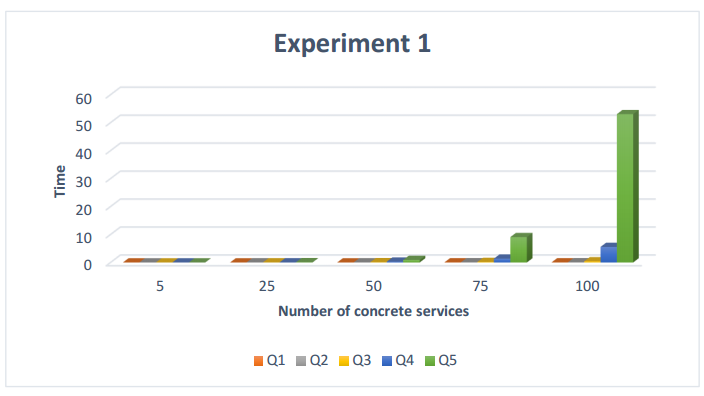
\includegraphics[scale=0.4]{exp1.png}
\caption{Query rewriting evaluation.}\label{fig01}
\end{figure} 

In the \textit{experiment 1}, there are five different queries that differ on the quantity of abstract services (increasing from 2 to 6). Analyzing the first experiment, it is easily to identify that the algorithm shares the same problem as existing query rewriting approaches using views: increasing the processing time when the size of the query and the number of concrete services increase. 

\begin{figure}[!h]
\centering
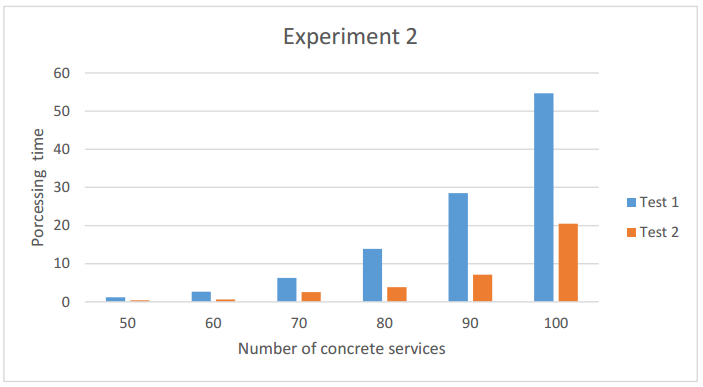
\includegraphics[scale=0.4]{exp2.png}
\caption{Query rewriting evaluation.}\label{fig02}
\end{figure} 

The \textit{experiment 2} presents the results considering our contribution regarding the use of user preferences and services' quality aspects extracted from SLAs to guide the service selection and query rewriting.
\textit{Test 1} and \textit{Test 2} include queries with six abstract services. 
The important difference between them is use of quality measures guiding the process. \textit{Test 1} do not consider quality measures as any other existing rewriting approach. On the other hand, \textit{Test 2} considers them.
The figure~\ref{fig02} shows our results. 

\begin{figure}[!h]
\centering
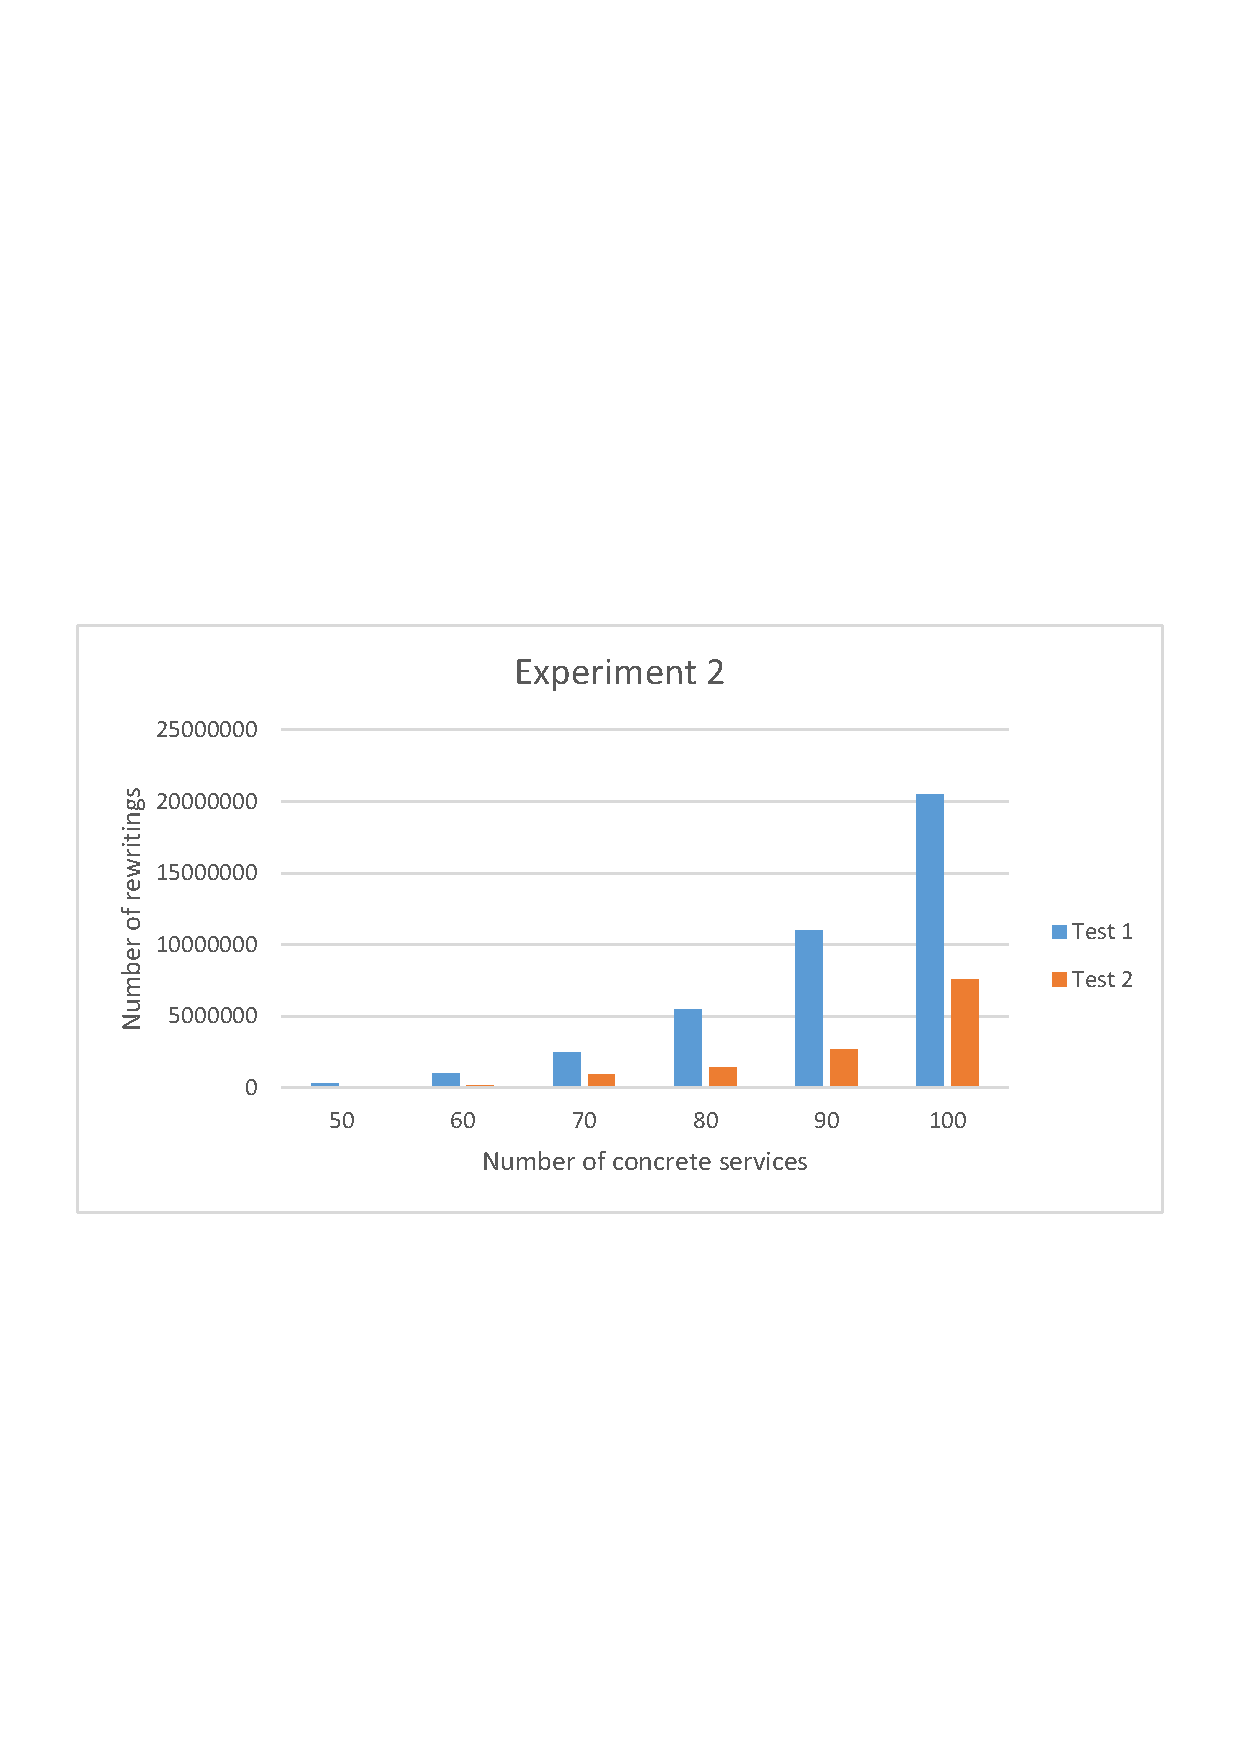
\includegraphics[scale=0.4]{exp3.png}
\caption{Query rewriting evaluation.}\label{fig03}
\end{figure} 

Analyzing the \textit{experiment 2} (figures~\ref{fig02} and \ref{fig03}), the results while considering the quality measures are promising.  
%The \textit{Rhone} presents a better performance, decreasing the processing time and 
%the total number of rewritings produced.  
%Reducing rewriting number allow to go straightforward to the rewriting solutions that are satisfactory avoiding any further backtrack.
The \textit{Rhone} increases performance reducing rewriting number (around 50 percent) which allows to go straightforward to the rewriting solutions that are satisfactory avoiding any further backtrack and thus reducing successful integration time.
\section{Final Remarks and Future Works}\label{sec:conclusion}
This work proposes a query rewriting algorithm for data integration quality
named \textit{Rhone}. Given a query, user preferences and a list of concrete services as input,
the algorithm derives rewritings in terms of concrete services that matches with the query and
fulfill the user preferences. The formalization and experiments are presented. The results 
show that the \textit{Rhone} reduces the rewriting number and processing time while considering 
user preferences and services' quality aspects extracted from SLAs to guide the service selection and rewriting.
We are currently performing improvements in the implementation and setting up a
multi-cloud simulation in in order to evaluate the performance of the
\textit{Rhone} in such context.  

 
\bibliographystyle{splncs03} 
\bibliography{bibliography}

\end{document}